We wish to approximate the solution to the heat equation 
\[ u_t(x,t) =  u_{xx}(x,t) + 100@t x, \qquad 0\le x \le 1,\ t\ge 0\]
with homogeneous Dirichlet boundary conditions
\[ u(0,t) = u(1,t) = 0\]
and initial condition
\[ u(x,0) = 0\]
using the finite element method (method of lines).
Let $N\ge 1$,  $h = 1/(N+1)$,  and $x_k = kh$ for $k = 0, \ldots, N+1$.
We shall construct approximations using the hat functions
\[ \phi_k(x) = \left\{ \begin{array}{ll}
           (x-x_{k-1})/h, & x\in [x_{k-1}, x_k);\\
           (x_{k+1}-x)/h, & x\in [x_k, x_{k+1});\\
            0,             & \mbox{otherwise}.
          \end{array}\right. \]
The approximate solution shall have the form
\[ u_N(x,t) = \sum_{k=1}^N a_k(t) \phi_k(x).\]

\begin{enumerate}
\item Write down the system of ordinary differential equations that determines
      the coefficients $a_k(t)$, $k=1,\ldots, N$.  Specify the
      entries in the mass and stiffness matrices and the load vector.\\
      (You may use results from previous homeworks and class as convenient.)

\item Write a MATLAB code that uses the backward Euler method
      to solve for the coefficients $a_k(t)$.\\
      Plot your approximate solution $u_N(x,t)$ at time $t = 1$.\\
      Choose $N$ and $\Delta t$ so that your solution appears to be accurate.\\
      Verify this accuracy by superimposing on your plot the computed
      solution at $t=1$ obtained by using space and time steps that are ten times smaller.

\end{enumerate}


%%%%%%%%%%%%%%%%%%%%%%%%%%%%%%%%%%%%%%%%%%%%%%%%%%%%%%%%%%%%%%%%%%%%%%%%%%%%%%%%

\ifthenelse{\boolean{showsols}}{\begin{solution}

\begin{enumerate}
\item
As derived in class, the system of ordinary differential equations 
that governs the behavior of the coefficients $a_k(t)$ is given by
\[ \BM {d \Ba \over d t} (t)  + \BK \Ba(t) = \Bf(t),\]
where $\BM$ and $\BK$ are the \emph{mass} and \emph{stiffness} matrices
whose $(j,k)$ entries are given by $(\phi_j,\phi_k)$ 
and $a(\phi_j,\phi_k)$.  
We also have
\[ \Ba(t) = \pmatrix{a_1(t)\cr a_2(t)\cr \vdots \cr a_N(t)}, \qquad
   \Bf(t) = \pmatrix{(f(\cdot,t),\phi_1) \cr 
                     (f(\cdot,t),\phi_2) \cr \vdots \cr
                     (f(\cdot,t),\phi_N)}. \]
When the basis functions $\{\phi_j\}_{j=1}^N$
are hat functions, we have
\[ \BM_{j,k} = (\phi_j,\phi_k) 
           = \left\{ \begin{array}{ll}
                   2h/3 & \mbox{if $j=k$;} \\
                   h/6  & \mbox{if $|j-k|=1$;} \\
                    0   & \mbox{otherwise.}
             \end{array}\right.,\]
as computed in Problem~3 of Problem Set~6, and
\[ \BK_{j,k} = a(\phi_j,\phi_k) 
           = \left\{ \begin{array}{ll}
                   2/h & \mbox{if $j=k$;} \\
                   -1/h  & \mbox{if $|j-k|=1$;} \\
                    0   & \mbox{otherwise.}
             \end{array}\right.,\]
as computed in class.

\item The backward Euler method for this differential equation 
      takes the form
      \[ \Ba_{k+1} = (\BI+\Delta t @\BM^{-1}\BK)^{-1} 
                     (\Ba_k + \Delta t @\BM^{-1} \Bf(t_{k+1})),\]
      which can be rearranged in the more computationally appealing form
      \[ \Ba_{k+1} = (\BM+\Delta t @\BK)^{-1} 
                     (\BM\Ba_k + \Delta t @\Bf(t_{k+1})).\]

      For this $f(x,t) = 100@t@x$, we have for fixed $t$ that
         \[ \Bf_j(t) = (f(\cdot,t), \phi_j) = 100@t@ \int_0^1 x \phi_j(x)\,dx,\]
      and (as can be readily computed with Mathematica)
         \[ \int_0^1 x \phi_j(x)\,dx 
               = \int_{x_{j-1}}^{x_j} {x (x-x_{j-1}) \over h}\, d x
                + \int_{x_j}^{x_{j+1}} {x(x_{j+1}-x)\over h}\, dx
               = \Big({hx_j \over 2} - {h^2\over 6}\Big)
                  + \Big({hx_j \over 2} + {h^2\over 6}\Big)
               = x_j h = jh^2.\] 

      The backward Euler method produces remarkably resilient solutions
      to this problem.
      The plot below compares the solution obtained the $N=8$ 
      and $\Delta t = 1/2$ (dots) to that
      computed with $N=80$ and $\Delta t = 1/20$.

\begin{center}
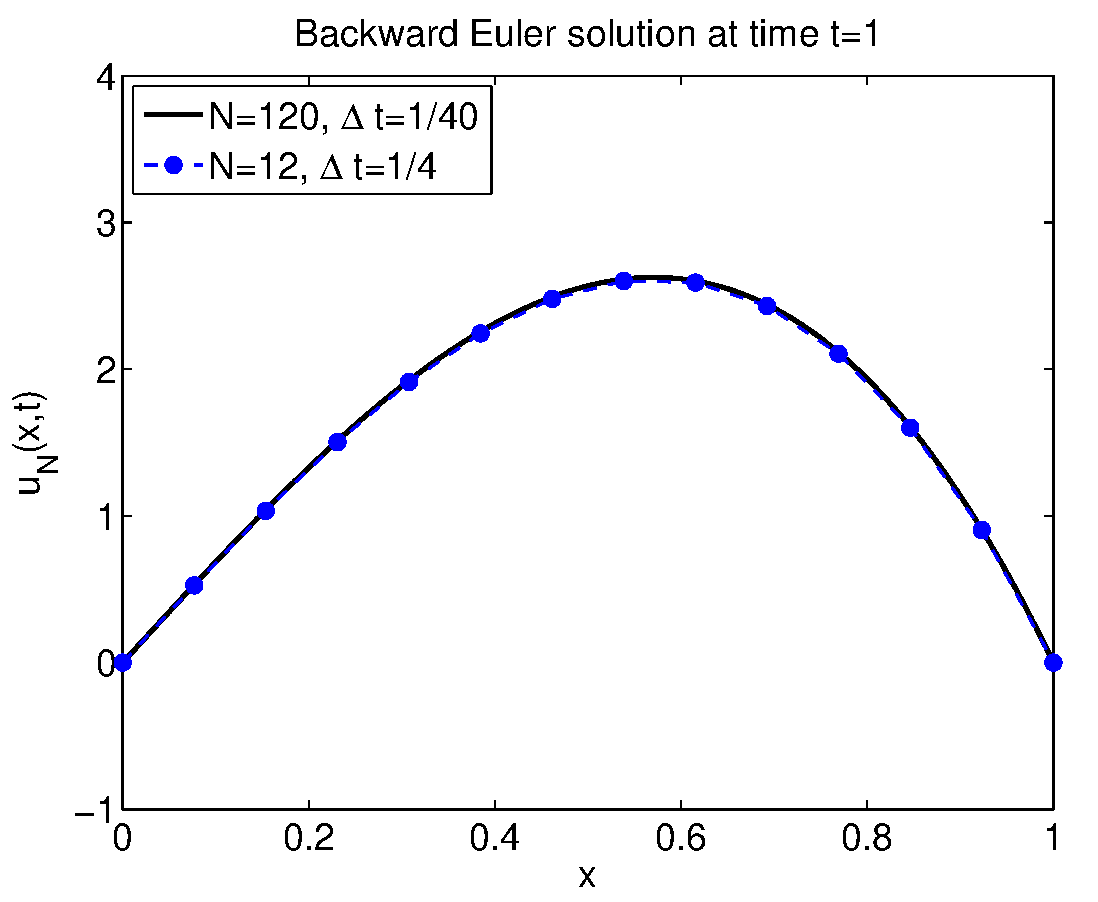
\includegraphics[scale=0.6]{femex1sol}
\end{center}

     MATLAB code to solve the problem for a specified $N$ and $\Delta t$
     is given below.

\input femex1code
\end{enumerate}
\end{solution}}{}

